\documentclass[11pt]{article}

\usepackage{pgfplots}
\usepgfplotslibrary{groupplots}
%\pgfplotsset{compat=1.14}

\usepackage{xcolor}

\definecolor{riptide}{RGB}{141,211,199}
\definecolor{pale_prim}{RGB}{255,255,179}
\definecolor{lavender_gray}{RGB}{190,186,218}
\definecolor{salmon}{RGB}{242,131,107}
\definecolor{seagull}{RGB}{128,177,211}
\definecolor{rajah}{RGB}{253,180,98}
\definecolor{yellow_green}{RGB}{198,222,119}
\definecolor{classic_rose}{RGB}{252,205,229}
\definecolor{feijoa}{RGB}{178,223,138}

\definecolor{cruise}{RGB}{179,226,205}
\definecolor{apricot}{RGB}{253,205,172}
\definecolor{periwinkle}{RGB}{203,213,232}
\definecolor{snow_flurry}{RGB}{230,245,201}
\definecolor{buttermilk}{RGB}{255,242,174}

\definecolor{sundown}{RGB}{249, 180, 181}
\definecolor{spindle}{RGB}{179,205,227}
\definecolor{tea_green}{RGB}{204,235,197}
\definecolor{languid_lavender}{RGB}{222,203,228}
\definecolor{champagne}{RGB}{254,217,166}
\definecolor{cream}{RGB}{255,255,204}


\definecolor{nonte_carlo}{RGB}{135,204,194}
\definecolor{melon}{RGB}{254,191,181}
\definecolor{granny_smith_apple}{RGB}{150,214,150}
\definecolor{mona_lisa}{RGB}{246,152,134}
\definecolor{watusi}{RGB}{254,221,207}
\definecolor{see_green}{RGB}{161,228,195}

\definecolor{moss_green}{RGB}{170,216,176}
\definecolor{opal}{RGB}{164,207,190}

\definecolor{pale_turquoise}{RGB}{172,240,242}
\definecolor{Madang}{RGB}{190,235,159}
\definecolor{pixie_green}{RGB}{183,214,170}
\definecolor{coral_andy}{RGB}{243,204,205}
\definecolor{manhattan}{RGB}{226,180,125}
\definecolor{quartz}{RGB}{219,223,238}
\definecolor{spring_sun}{RGB}{242,243,195}
\definecolor{dairy_cream}{RGB}{254,226,189}
\definecolor{surf_crest}{RGB}{205,230,208}
\definecolor{french_pass}{RGB}{195,232,246}
\definecolor{cosmos}{RGB}{248,209,210}
\definecolor{portafino}{RGB}{245,237,160}
\definecolor{sail}{RGB}{163,205,235}
\definecolor{hint_green}{RGB}{226,246,209}


\definecolor{jet_stream}{RGB}{188, 214, 210}


\definecolor{azalea}{RGB}{251, 196, 196}
\definecolor{wewak}{RGB}{244, 143, 150}
\definecolor{bittersweet}{RGB}{255,111,105}
\definecolor{sunset_orange}{RGB}{242,89,75}
\definecolor{light_coral}{RGB}{244, 127, 123}
\definecolor{carnation}{RGB}{245, 80, 86}
\definecolor{flamingo}{RGB}{237, 88, 85}
\definecolor{carmine_pink}{RGB}{231, 76, 60}
\definecolor{deep_carmine_pink}{RGB}{236, 50, 67}
\definecolor{fire_engine_red}{RGB}{210,44,41}
\definecolor{amaranth}{RGB}{234,46,73}
\definecolor{ku_crimson}{RGB}{243, 0, 25}
\definecolor{fire_engine_red}{RGB}{206, 37, 51}
\definecolor{copper_rust}{RGB}{155, 64, 74}

\definecolor{chilean_fire}{RGB}{215, 87, 44}

\definecolor{japanese_laurel}{RGB}{53, 116, 40}


\definecolor{turmeric}{RGB}{211, 178, 76}
\definecolor{saffron}{RGB}{249,193,62}
\definecolor{my_sin}{RGB}{255, 176, 59}
\definecolor{tree_poppy}{RGB}{246, 154, 27}
\definecolor{jaffa}{RGB}{240, 131, 58}
\definecolor{crusta}{RGB}{254, 127, 44}
\definecolor{tahiti_gold}{RGB}{223, 102, 36}
\definecolor{outrageous_orange}{RGB}{255, 100, 45}
\definecolor{safety_orange}{RGB}{254, 106, 0}



\definecolor{turquoise}{RGB}{41,217,194}
\definecolor{puerto_rico}{RGB}{94, 194, 166}
\definecolor{mountain_meadow}{RGB}{0, 163, 136}
\definecolor{free_speech_aquamarine}{RGB}{0, 156, 114}
\definecolor{java}{RGB}{2,190,196}


% person:
\definecolor{matisse}{RGB}{25, 104, 167}
\definecolor{shakespeare}{RGB}{85, 154, 193}
\definecolor{mona_lisa}{RGB}{246,152,134}

% gray:
\definecolor{bgc}{RGB}{245,245,245}
\definecolor{tuatara}{RGB}{67, 67, 67}
\definecolor{aluminum}{RGB}{153,153,153}
\definecolor{silver}{RGB}{191,191,191}
\definecolor{platinum}{RGB}{228,228,228}
\definecolor{mercury}{RGB}{230,230,230}
\definecolor{gallery}{RGB}{240,240,240}
\definecolor{athens_gray}{RGB}{236, 240, 241}

% nature color
\definecolor{early_dawn}{RGB}{252,243,218}
\definecolor{egg_shell}{RGB}{238, 234, 215}
\definecolor{midnight}{RGB}{0, 29, 50}
\definecolor{sundown}{RGB}{249, 180, 181}
\definecolor{sun_shade}{RGB}{255, 144, 68}
\definecolor{sushi}{RGB}{117, 168, 47}
\definecolor{tomato}{RGB}{255, 97, 56}
\definecolor{ice_cold}{RGB}{169,232,220}


% blue:
\definecolor{jelly_bean}{RGB}{45, 126, 150}
\definecolor{shakespeare}{RGB}{85, 154, 193}
\definecolor{celestial_blue}{RGB}{52, 152, 219}
\definecolor{curious_blue}{RGB}{41, 128, 185}
\definecolor{french_blue}{RGB}{0, 112, 182}
\definecolor{matisse}{RGB}{25, 104, 167}

\definecolor{biscay}{RGB}{44, 62, 80}

% green:
\definecolor{cosmic_latte}{RGB}{222, 247, 229}
\definecolor{chinook}{RGB}{163, 232, 178}
\definecolor{padua}{RGB}{121, 189, 143}
\definecolor{ocean_green}{RGB}{79, 176, 112}
\definecolor{pastel_green}{RGB}{107, 227, 135}
\definecolor{chateau_green}{RGB}{69, 191, 85}
\definecolor{RoyalBlue}{RGB}{69, 191, 85}
\definecolor{pigment_green}{RGB}{0, 175, 79}
\definecolor{fern}{RGB}{101,197,117}
\definecolor{killarney}{RGB}{56, 113, 66}
\definecolor{viridian}{RGB}{70, 137, 102}


\definecolor{jet_stream}{rgb}{0.69,0.61,0.85}
\definecolor{jelly_bean}{rgb}{0.47,0.32,0.66}




\begin{document}


\pgfplotsset{
axis background/.style={fill=gallery},
grid=both,
  xtick pos=left,
  ytick pos=left,
  tick style={
    major grid style={style=white,line width=1pt},
    minor grid style=bgc,
    draw=none
    },
  minor tick num=1,
  ymajorgrids,
	major grid style={draw=white},
	y axis line style={opacity=0},
	tickwidth=0pt,
}
%nodes near coords,
%every node near coord/.append style={anchor=north, font=\fontsize{4pt}{4pt}\selectfont},%\fontsize{4pt}{4pt}\selectfont
%every tick label/.append style={font=\scriptsize}

%diamond*, triangle*, square, pentagon, *

\begin{figure}
\centering
    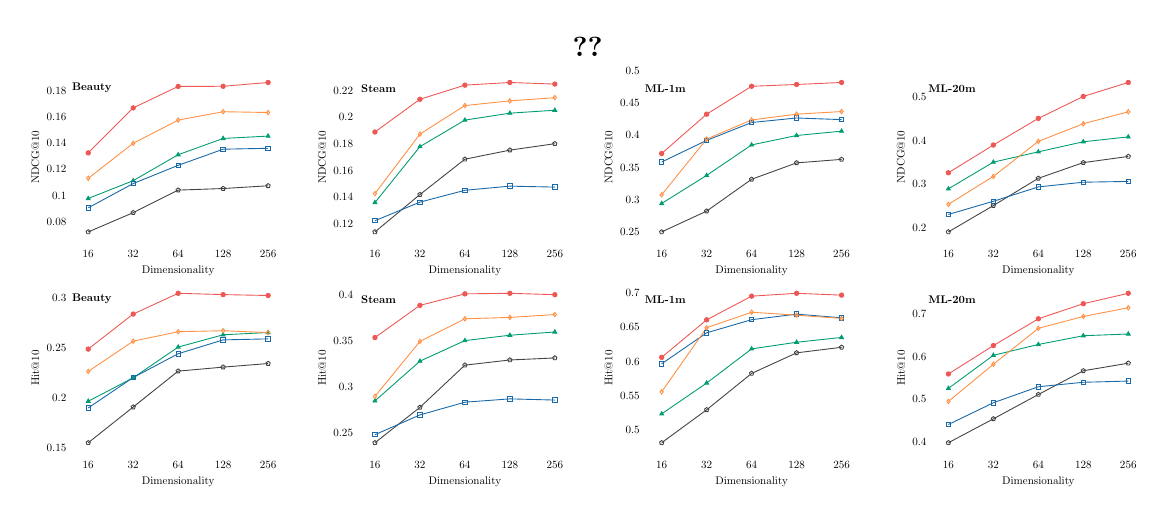
\begin{tikzpicture}[scale=0.4]
	\begin{groupplot}[
	    group style={group size=4 by 2,
	        horizontal sep = 64pt
	        }, 
%	    width=0.5\textwidth,
%	    height=0.4\textwidth,
	    xlabel=Dimensionality,
        ylabel=NDCG@10,
        xticklabels={16, 32, 64, 128, 256},
        xtick={1,2,3,4,5},
        ymajorgrids,
        major grid style={draw=white},
        y axis line style={opacity=0},
        tickwidth=0pt,
        yticklabel style={
        /pgf/number format/fixed,
        /pgf/number format/precision=5
        },
        scaled y ticks=false,
        every axis title/.append style={at={(0.1,0.8)},font=\bfseries}
	    ]
		\nextgroupplot[
		legend style = {
		  font=\small,
          draw=none, 
          fill=none,
          column sep = 2pt, 
          /tikz/every even column/.append style={column sep=5mm},
          legend columns = -1, 
          legend to name = grouplegend},
		title=Beauty, 
%		ymin = 0.05,
%		ymax = 0.2,
		]
		
		\addplot[thick,color=tuatara,mark=pentagon] coordinates {
          (1, 0.0722)
          (2, 0.0869)
          (3, 0.1041)
          (4, 0.1053)
          (5, 0.1074)
        }; \addlegendentry{GRU4Rec}
         \addplot[thick,color=free_speech_aquamarine,mark=triangle*] coordinates {
          (1, 0.0977)
          (2, 0.1113)
          (3, 0.1311)
          (4, 0.1435)
          (5, 0.1453)
        }; \addlegendentry{GRU4Rec$^{+}$}
        \addplot[thick,color=matisse,mark=square] coordinates {
          (1, 0.0906)
          (2, 0.1091)
          (3, 0.1230)
          (4, 0.1353)
          (5, 0.1360)
        };\addlegendentry{Caser}
        \addplot[thick,color=sun_shade,mark=diamond] coordinates {
          (1, 0.1131)
          (2, 0.1398)
          (3, 0.1575)
          (4, 0.1639)
          (5, 0.1633)
        };\addlegendentry{SASRec}
        \addplot[thick,color=flamingo,mark=*] coordinates {
          (1, 0.1325)
          (2, 0.1668)
          (3, 0.1832)
          (4, 0.1833)
          (5, 0.1862)
        };\addlegendentry{BERT4Rec}
        
        \nextgroupplot[
        title=Steam]
		\addplot[thick,color=tuatara,mark=pentagon] coordinates {
          (1, 0.1141)
          (2, 0.1421)
          (3, 0.1686)
          (4, 0.1754)
          (5, 0.1802)
        };
         \addplot[thick,color=free_speech_aquamarine,mark=triangle*] coordinates {
          (1, 0.1361)
          (2, 0.1780)
          (3, 0.1979)
          (4, 0.2031)
          (5, 0.2053)
        };
        \addplot[thick,color=matisse,mark=square] coordinates {
          (1, 0.1225)
          (2, 0.1364)
          (3, 0.1453)
          (4, 0.1484)
          (5, 0.1477)
        };
        \addplot[thick,color=sun_shade,mark=diamond] coordinates {
          (1, 0.1428)
          (2, 0.1874)
          (3, 0.2088)
          (4, 0.2123)
          (5, 0.2147)
        };
        \addplot[thick,color=flamingo,mark=*] coordinates {
          (1, 0.1890)
          (2, 0.2135)
          (3, 0.2241)
          (4, 0.2261)
          (5, 0.2249)
        };
        
        \nextgroupplot[title=ML-1m]
		\addplot[thick,color=tuatara,mark=pentagon] coordinates {
          (1, 0.2504)
          (2, 0.2826)
          (3, 0.3319)
          (4, 0.3573)
          (5, 0.3627)
        };
         \addplot[thick,color=free_speech_aquamarine,mark=triangle*] coordinates {
          (1, 0.2944)
          (2, 0.3379)
          (3, 0.3851)
          (4, 0.3997)
          (5, 0.4064)
        };
        \addplot[thick,color=matisse,mark=square] coordinates {
          (1, 0.3587)
          (2, 0.3921)
          (3, 0.4198)
          (4, 0.4268)
          (5, 0.4243)
        };
        \addplot[thick,color=sun_shade,mark=diamond] coordinates {
          (1, 0.3080)
          (2, 0.3941)
          (3, 0.4238)
          (4, 0.4327)
          (5, 0.4368)
        };
        \addplot[thick,color=flamingo,mark=*] coordinates {
          (1, 0.3718)
          (2, 0.4327)
          (3, 0.4759)
          (4, 0.4787)
          (5, 0.4818)
        };
        
        \nextgroupplot[title=ML-20m]
		\addplot[thick,color=tuatara,mark=pentagon] coordinates {
          (1, 0.1900)
          (2, 0.2506)
          (3, 0.3134)
          (4, 0.3495)
          (5, 0.3637)
        };
         \addplot[thick,color=free_speech_aquamarine,mark=triangle*] coordinates {
          (1, 0.2891)
          (2, 0.3506)
          (3, 0.3743)
          (4, 0.3975)
          (5, 0.4087)
        };
        \addplot[thick,color=matisse,mark=square] coordinates {
          (1, 0.2302)
          (2, 0.2605)
          (3, 0.2936)
          (4, 0.3044)
          (5, 0.3062)
        };
        \addplot[thick,color=sun_shade,mark=diamond] coordinates {
          (1, 0.2535)
          (2, 0.3177)
          (3, 0.3984)
          (4, 0.4390)
          (5, 0.4665)
        };
        \addplot[thick,color=flamingo,mark=*] coordinates {
          (1, 0.3261)
          (2, 0.3900)
          (3, 0.4513)
          (4, 0.5018)
          (5, 0.5340)
        };
        
        
        \nextgroupplot[
        title=Beauty,
        ylabel=Hit@10]
		\addplot[thick,color=tuatara,mark=pentagon] coordinates {
          (1, 0.1549)
          (2, 0.1907)
          (3, 0.2267)
          (4, 0.2307)
          (5, 0.2343)
        };
         \addplot[thick,color=free_speech_aquamarine,mark=triangle*] coordinates {
          (1, 0.1965)
          (2, 0.2200)
          (3, 0.2508)
          (4, 0.2631)
          (5, 0.2654)
        };
        \addplot[thick,color=matisse,mark=square] coordinates {
          (1, 0.1898)
          (2, 0.2203)
          (3, 0.2441)
          (4, 0.2580)
          (5, 0.2590)
        };
        \addplot[thick,color=sun_shade,mark=diamond] coordinates {
          (1, 0.2264)
          (2, 0.2567)
          (3, 0.2662)
          (4, 0.2672)
          (5, 0.2653)
        };
        \addplot[thick,color=flamingo,mark=*] coordinates {
          (1, 0.2488)
          (2, 0.2839)
          (3, 0.3047)
          (4, 0.3034)
          (5, 0.3025)
        };
        
        \nextgroupplot[
        title=Steam,
        ylabel=Hit@10]
		\addplot[thick,color=tuatara,mark=pentagon] coordinates {
          (1, 0.2395)
          (2, 0.2778)
          (3, 0.3235)
          (4, 0.3291)
          (5, 0.3313)
        };
         \addplot[thick,color=free_speech_aquamarine,mark=triangle*] coordinates {
          (1, 0.2848)
          (2, 0.3278)
          (3, 0.3501)
          (4, 0.3559)
          (5, 0.3594)
        };
        \addplot[thick,color=matisse,mark=square] coordinates {
          (1, 0.2482)
          (2, 0.2696)
          (3, 0.2834)
          (4, 0.2870)
          (5, 0.2857)
        };
        \addplot[thick,color=sun_shade,mark=diamond] coordinates {
          (1, 0.2897)
          (2, 0.3492)
          (3, 0.3737)
          (4, 0.3752)
          (5, 0.3783)
        };
        \addplot[thick,color=flamingo,mark=*] coordinates {
          (1, 0.3534)
          (2, 0.3882)
          (3, 0.4007)
          (4, 0.4013)
          (5, 0.3998)
        };
        
        \nextgroupplot[
        title=ML-1m,
        ylabel=Hit@10]
		\addplot[thick,color=tuatara,mark=pentagon] coordinates {
          (1, 0.4811)
          (2, 0.5293)
          (3, 0.5825)
          (4, 0.6126)
          (5, 0.6207)
        };
         \addplot[thick,color=free_speech_aquamarine,mark=triangle*] coordinates {
          (1, 0.5233)
          (2, 0.5684)
          (3, 0.6184)
          (4, 0.6281)
          (5, 0.6351)
        };
        \addplot[thick,color=matisse,mark=square] coordinates {
          (1, 0.5966)
          (2, 0.6419)
          (3, 0.6611)
          (4, 0.6692)
          (5, 0.6639)
        };
        \addplot[thick,color=sun_shade,mark=diamond] coordinates {
          (1, 0.5556)
          (2, 0.6493)
          (3, 0.6720)
          (4, 0.6677)
          (5, 0.6629)
        };
        \addplot[thick,color=flamingo,mark=*] coordinates {
          (1, 0.6060)
          (2, 0.6609)
          (3, 0.6955)
          (4, 0.6997)
          (5, 0.6970)
        };
        
        \nextgroupplot[
        title=ML-20m,
        ylabel=Hit@10]
		\addplot[thick,color=tuatara,mark=pentagon] coordinates {
          (1, 0.3990)
          (2, 0.4547)
          (3, 0.5114)
          (4, 0.5667)
          (5, 0.5844)
        };
         \addplot[thick,color=free_speech_aquamarine,mark=triangle*] coordinates {
          (1, 0.5257)
          (2, 0.6028)
          (3, 0.6280)
          (4, 0.6484)
          (5, 0.6524)
        };
        \addplot[thick,color=matisse,mark=square] coordinates {
          (1, 0.4415)
          (2, 0.4922)
          (3, 0.5295)
          (4, 0.5399)
          (5, 0.5427)
        };
        \addplot[thick,color=sun_shade,mark=diamond] coordinates {
          (1, 0.4953)
          (2, 0.5819)
          (3, 0.6657)
          (4, 0.6933)
          (5, 0.7136)
        };
        \addplot[thick,color=flamingo,mark=*] coordinates {
          (1, 0.5593)
          (2, 0.6254)
          (3, 0.6879)
          (4, 0.7230)
          (5, 0.7473)
        };
        
	\end{groupplot}
\node at ($(group c1r1) + (370pt, 100pt)$) {\ref{grouplegend}};
\end{tikzpicture}
    \caption{Example for groupplot and line chart.}
    \label{fig:example}
\end{figure}


\end{document}
